\section{Notas musicais, tons e escalas}\index{Música!Notas musicais}
\label{sec:notasmusicais}

O sons musicais que representam as notas são sete, 
e foram designadas pelos gregos com as sete primeiras letras do alfabeto,
estes são: \{A, B, C, D, E, F, G\} \cite[pp. 11]{grabner2001teoria} \cite[pp. 9]{cardoso1973curso}.
O ocidente adotou esta forma porem no século XI, 
Guido d'Arezzo rebatizou as notas, 
atribuindo a cada nota a primeira sílaba dos versos
de um hino a São Jõao muito conhecido na época:
\begin{citando}%%
\textbf{Ut} queant laxls,\\
\textbf{re}sonare fibris,\\
\textbf{Mi}ra gestorum,\\
\textbf{fa}muli tuorum,\\
\textbf{Sol}ve polluti,\\
\textbf{La}bii reatum,\\
\textbf{S}ánete lohannes.
\end{citando}
 Assim, apos a troca de ``ut'' por ``do'' nascem as notas musicais: 
\{lá, si, dó, ré, mi, fá, sol\} \cite[pp. 21]{arbones2012armonia} \cite[pp. 7]{cardoso1973curso}. 
A Tabela \ref{tab:notasmusic} mostra a relação entre estas duas notações.

\begin{table}[h]
\centering
\begin{tabular}{|c|c|c|c|c|c|c|}
\hline
A  & B  & C  & D  & E  & F  & G\\ \hline
lá & si & dó & ré & mi & fá & sol \\ \hline
\end{tabular}
\caption{Notas musicais}
\label{tab:notasmusic}
\end{table}

Estas sete notas representam sons com \hyperref[sec:pos:Altura]{\textbf{alturas}} diferentes.
Porem, existem varias formas de atribuir uma \hyperref[sec:pos:Altura]{\textbf{altura}} 
especifica a cada uma destas notas, 
sendo a mais difundida atualmente a afinação (atribuição de alturas) com \hyperref[subsec:tempigual]{\textbf{temperamento igual}}\footnote{O temperamento igual é tratado na Seção \ref{subsec:tempigual}.}.


%%%%%%%%%%%%%%%%%%%%%%%%%%%%%%%%%%%%%%%%%%%%%%%%%%%%%%%%%%%%%%%%%%%%%%%%%%%%%%%%
\subsection{Escalas musicais}

\label{sec:pos:Escala}
\index{Música!Escalas musicais}
As escalas musicais são uma forma de organizar as notas musicais, 
numa ordem que permitam ser lidas de forma crescente em relação a altura dos sons.
Existe uma variedade de escalas musicais usadas em distintas épocas ou países, 
porem a escala básica da música europeia é a escala diatônica. \cite[pp. 753]{apel1969harvard}
\begin{example}As escalas mais conhecidas são:
\begin{inparaitem}
\item Escala diatônica
\item Escala cromática
%\item Escala diatônica no modo jônico
%\item Escala diatônica no modo dórico
%\item Escala diatônica no modo frígio
%\item Escala diatônica no modo lídio
%\item Escala diatônica no modo mixolídio
%\item Escala diatônica no modo eólico
%\item Escala diatônica no modo lócrio
\item Escala pentatônica
\item Escala de blues
\item etc.
\end{inparaitem}
\end{example}

\begin{description}

\item [Escala diatônica:] \label{sec:pos:Diatonica}
\index{Música!Escala diatônica}
Também conhecida como \textbf{escala de C-major},
é uma sucessão de 8 sons,  escritos em sentido ascendente em relação a altura das notas, 
sendo os 7 primeiros sons as notas mostradas na Tabela \ref{tab:notasmusic}, iniciando em dó,
e a oitava nota a repetição da primeira nota, 
porem mais aguda, é dizer com uma frequência igual ao dobro.
Existem 7 distancias entre as 8 notas, medidas em progressão geométrica\footnote{A 
distancia, em progressão geométrica, entre dois números $X$ e $Y$, é obtida calculando o fator $\frac{Y}{X}$. }, 
sendo que estas distancias tem só dois longitudes diferentes, chamadas tons e semitons;
de modo que a separação entre as notas nesta escala é distribuída da seguinte forma: 
tom,tom,semitom,tom,tom,tom,semitom \cite[pp. 30]{cardoso1973curso}\cite[pp. 753]{apel1969harvard}.
\begin{example}
\begin{equation*}
d\acute{o}\overset{tom}{\rightarrow}
r\acute{e}\overset{tom}{\rightarrow}
mi\overset{semitom}{\rightarrow}
f\acute{a}\overset{tom}{\rightarrow}
sol\overset{tom}{\rightarrow}
l\acute{a}\overset{tom}{\rightarrow}
si\overset{semitom}{\rightarrow}
d\acute{o}
\end{equation*}
\end{example}
Para mais detalhes numéricos da escala diatônica ir a Página \pageref{ref:paginadiatonicanumerica}.


\item [Escala cromática:] \label{sec:pos:Cromatica}
\index{Música!Escala cromática}
Também chamada escala dodecafônica ou duodécuple, 
esta escala está constituída por uma sucessão de 12 sons, separados uma distancia de 1 semitom.
Os outros tipos de escalas na música moderna podem ser considerados como subconjuntos desta escala \cite[pp. 753]{apel1969harvard}
\begin{example} 
Se representamos um semitom por ``$\alpha$'', 
e definimos o simbolo $\#$ como indicador de uma nota, um semitom acima, 
então a escala cromática é definida como:\\
$d\acute{o}\overset{\alpha}{\rightarrow}$
$\#d\acute{o}\overset{\alpha}{\rightarrow}$
$r\acute{e}\overset{\alpha}{\rightarrow}$
$\#r\acute{e}\overset{\alpha}{\rightarrow}$
$mi\overset{\alpha}{\rightarrow}$
$f\acute{a}\overset{\alpha}{\rightarrow}$
$\#f\acute{a}\overset{\alpha}{\rightarrow}$
$sol\overset{\alpha}{\rightarrow}$
$\#sol\overset{\alpha}{\rightarrow}$
$l\acute{a}\overset{\alpha}{\rightarrow}$
$\#l\acute{a}\overset{\alpha}{\rightarrow}$
$si$
\end{example}

\end{description}~\\


%%%%%%%%%%%%%%%%%%%%%%%%%%%%%%%%%%%%%%%%%%%%%%%%%%%%%%%%%%%%%%%%%%%%%%%%%%%%%%%%
\subsection{Tom e Semitom}
\label{subsec:tomesemitom}
\index{Música!Tom}
\index{Música!Semitom}

Os tons e semitons são termos usados para designar aos intervalos entre as alturas das notas utilizados na 
\hyperref[sec:pos:Diatonica]{\textbf{escala diatônica}}.
Deve-se ter em conta que quando usamos o nome tom,
podemos nos referir a \hyperref[sec:pos:Altura]{\textbf{altura}} 
de uma nota ou ao intervalo entre algumas notas da escala diatônica;
a continuação usaremos esta última acepção.

\begin{description}

\item [Semitom:] \label{sec:pos:Semitom}
\index{Música!Semitom}
É a menor distancia entre duas notas na música tradicional ocidental.
Na \hyperref[sec:pos:Diatonica]{\textbf{escala diatônica}} 
podem se achar distancias de semitons entre mi e fá, e entre si e dó.
O valor exato de um semitom varia ligeiramente de acordo com o sistema de afinação \cite[pp. 30]{cardoso1973curso}\cite[pp. 762]{apel1969harvard}, ver afinação com temperamento igual na Seção \ref{subsec:tempigual}. 
Em algumas bibliografias se define ao semitom como a ``metade'' de um tom, 
porem esta só é uma forma metafórica de falar, 
pois um semitom não representa a metade do valor numérico de um tom;
em verdade os tons e semitons são calculados considerando que as notas cumprem uma progressão geométrica
(irregular na escala diatônica e regular na escala cromática);
assim, o correto seria falar que: um semitom está na metade do caminho, em progressão geométrica, de um tom\footnote{Na 
afinação com temperamento igual um $Semitom=\sqrt{tom}$}.
\begin{example}
Se numa escala diatônica definimos $f_{mi}$ e $f_{fa}$ como as frequências das notas mi e fá respetivamente.
então o valor de um semitom seria equivalente a,
\begin{equation*}
Semitom=\frac{f_{fa}}{f_{mi}}
\end{equation*}
\end{example}

\item [Tom:] \label{sec:pos:TomDist}
\index{Música!Tom}
É uma distancia, em progressão geométrica, equivalente a duas distancias de semitons colocadas consecutivamente entre duas notas.
Na \hyperref[sec:pos:Diatonica]{\textbf{escala diatônica}} podemos achar distancias de um tom entre todas as notas exceto entre mi e fá, e entre si e dó \cite[pp. 30]{cardoso1973curso}\cite[pp. 762]{apel1969harvard}.
O valor exato de um tom varia ligeiramente de acordo com o sistema de afinação, ver afinação com temperamento igual na Seção \ref{subsec:tempigual}. 
\begin{example}
Se numa escala diatônica definimos $f_{fa}$ e $f_{sol}$ como as frequências das notas fá e sol respetivamente.
então o valor de um tom seria equivalente a,
\begin{equation*}
Tom=\frac{f_{sol}}{f_{fa}}
\end{equation*}
\end{example}

\item [Oitava:] \label{sec:pos:Oitava}
\index{Música!Oitava}
Representa o oitavo tom de uma \hyperref[sec:pos:Diatonica]{\textbf{escala diatônica}}. 
Correspondente  ao tom com o dobro da frequência do tom escolhido como referencia \cite[pp. 589]{apel1969harvard}
\begin{example}~
\begin{itemize}
\item Dado uma nota lá a $440$ hertz, teremos um lá numa oitava superior a uma frequência de $880$ hertz  
\item Dado uma nota lá a $440$ hertz, teremos um lá numa oitava inferior a uma frequência de $220$ hertz  
\end{itemize}
\end{example}

\end{description}~\\

%%%%%%%%%%%%%%%%%%%%%%%%%%%%%%%%%%%%%%%%%%%%%%%%%%%%%%%%%%%%%%%%%%%%%%%%%%%%%%%%
\subsection{Acidentes ou alterações}
\label{subsec:acidentes}
\index{Música!Acidentes}


Os acidentes ou alterações são símbolos que modificam a altura de uma nota; 
os mais utilizado são \cite[pp. ]{alves2004teoria}:\\

\begin{description}

\item [Sustenido ($\#$):] \label{sec:pos:Sustenido}
\index{Música!Sustenido}
É um simbolo u operador que acompanha a uma nota, 
e indica um som com uma altura um semitom acima da nota indicada.
Uma vez usado o símbolo, o âmbito  do simbolo continua ativo, 
para notas do mesmo tom, sem a necessidade de grafar novamente com o símbolo $\#$;
para desabilitar este âmbito, se usa o simbolo $\natural$. 
\begin{example} $\#$dó : é equivalente a dizer, um som um semitom acima de dó.
\end{example}


\item [Bemol ($\flat$):] \label{sec:pos:Bemol}
\index{Música!Bemol}
É um simbolo u operador que acompanha a uma nota, 
e indica um som com uma altura um semitom abaixo da nota indicada. 
Uma vez usado o símbolo, o âmbito  do simbolo continua ativo, 
para notas do mesmo tom, sem a necessidade de grafar novamente com o símbolo $\flat$;
para desabilitar este âmbito, se usa o simbolo $\natural$. 
\begin{example} $\flat$ré : é equivalente a dizer, um som um semitom abaixo de ré.
\end{example}

\item [Bequadro ($\natural$):] \label{sec:pos:Bequadro}
\index{Música!Bequadro}
Este símbolo anula o efeito dos símbolos anteriormente mencionados.

\end{description}~\\

%%%%%%%%%%%%%%%%%%%%%%%%%%%%%%%%%%%%%%%%%%%%%%%%%%%%%%%%%%%%%%%%%%%%%%%%%%%%%%%%
\subsection{Temperamento igual}
\label{subsec:tempigual}
\index{Música!Temperamento igual}
No  temperamento igual se divide uma oitava em doze semitons da mesma distancia.
de modo que qualquer par de notas separadas uma 
\hyperref[sec:pos:Oitava]{\textbf{oitava}} tenham uma distancia igual a $2$ \cite[pp. 835]{apel1969harvard}.
Assim, se temos um par de notas lá, a primeira a uma frequência $f_0$, 
e a outra uma oitava acima com uma frequência $2f_0$;
e sabendo que existem $12$ passos (semitons) em progressão  geométrica para completar uma oitava 
(como mostra a Tabela \ref{tab:temperamento1} na linha 4),
então a distancia $\alpha$ de cada semitom pode ser calculada como:
\begin{equation}
f_0\alpha^{12}\equiv 2 f_0
\end{equation}
\begin{sidewaystable}
\centering
\begin{tabular}{|c|c|c|c|c|c|c|c|c|c|c|c||c|}
\hline
 lá  & ~ & si  & dó  & ~ & ré  & ~ & mi  & fá  & ~ & sol   & ~ & lá\\ \hline
 ~  & $\#$lá  & ~  & ~  & $\#$dó  & ~  & $\#$ré  & ~  & ~  & $\#$fá  & ~   & $\#$sol   & ~\\ \hline
 ~  & $\flat$si  & ~  & ~  &  $\flat$ré  & ~  &  $\flat$mi  & ~  & ~  &  $\flat$sol  & ~   &  $\flat$lá   & ~\\ \hline
$f_0$ & $f_0\alpha$ & $f_0\alpha^2$ & $f_0\alpha^3$ & $f_0\alpha^4$ & $f_0\alpha^5$ & $f_0\alpha^6$ & $f_0\alpha^7$ & $f_0\alpha^8$ & $f_0\alpha^9$ & $f_0\alpha^{10}$ & $f_0\alpha^{11}$ & $f_0\alpha^{12}$ \\ \hline
\end{tabular}
\caption{Temperamento igual em todas as notas da escala cromática.}
\label{tab:temperamento1}
\end{sidewaystable}
de modo que um \hyperref[sec:pos:Semitom]{\textbf{semitom}} ($\alpha$) é igual a,
\begin{equation}
\alpha \equiv \sqrt[12]{2} \approx  1.05946309435930,
\end{equation}
e um \hyperref[sec:pos:TomDist]{\textbf{tom}} ($\alpha^2$) é igual a,
\begin{equation}
\alpha^2 \equiv \sqrt[6]{2} \approx  1.12246204830937,
\end{equation}

Assim, para qualquer nota selecionada na escala, 
se cumpre que a frequência se duplica apos 12 semitons.
No caso da Figura \ref{fig:circulonotas} isto é valido quando avançamos no sentido das agulhas do relógio.
Por outro lado, a frequência se dividirá por dois a cada 12 semitons,
em sentido contrario as agulhas do relógio.
    \begin{figure}[h]
        \centering
        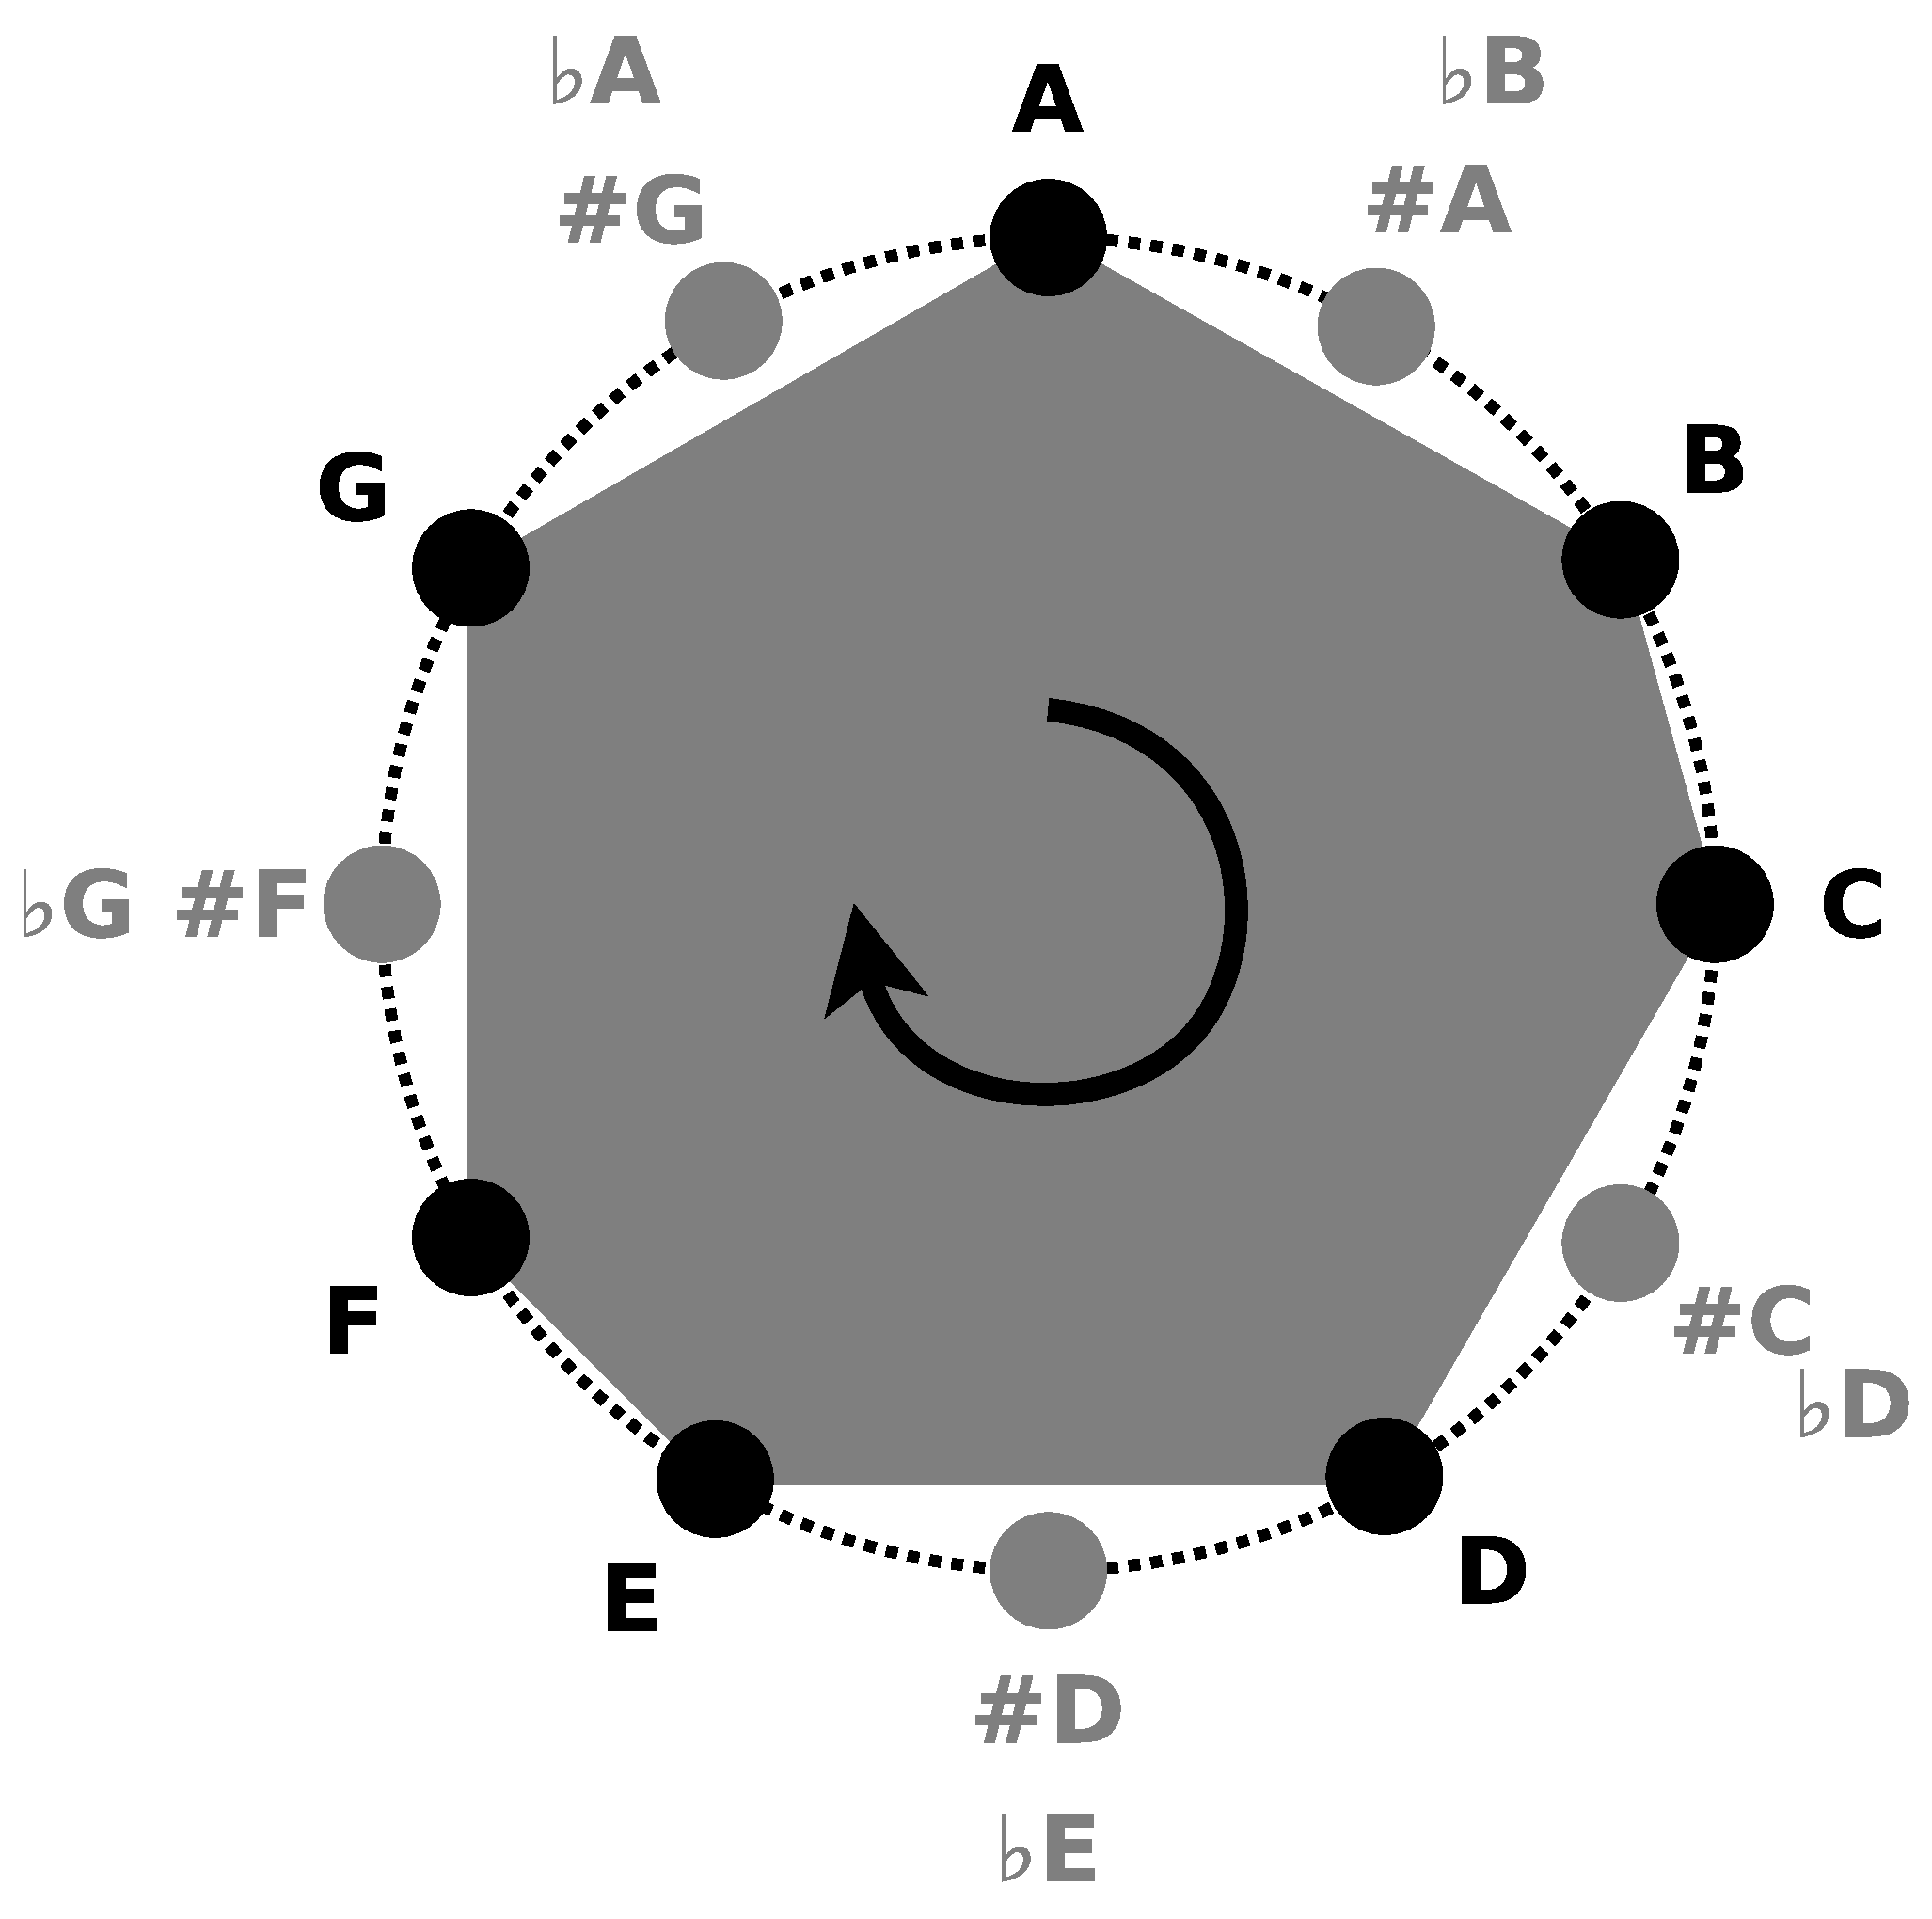
\includegraphics[width=0.65\textwidth]{chapters/cap-musica-basica/circulonotas.eps}
        \caption{Representação cíclica das distancias das notas musicais.}
        \label{fig:circulonotas}
    \end{figure}

Adicionalmente, na Figura \ref{fig:circulonotas}, 
está representada a escala diatônica com uma figura geométrica de 6 lados, 
colorido em cinza; e a escala cromática está representada com um circulo de linha pontuada.


